\section{Introduction to problem}
\frame{\sectionpage} % this adds the slide with the section title, if you don't want that slide included you can remove it.
    
\begin{frame}{Introduction}
\begin{itemize}
    \item Itemize lets you add bullets to your document like this.
    \item You can have as many bullets as will fit on a page.
\end{itemize}
\end{frame}

\begin{frame}{Including figures}
You can add figures/images to the document the same as you do in any latex document.  

\begin{figure}[H]
     \centering
     \begin{subfigure}[b]{0.49\linewidth}
        \centering
        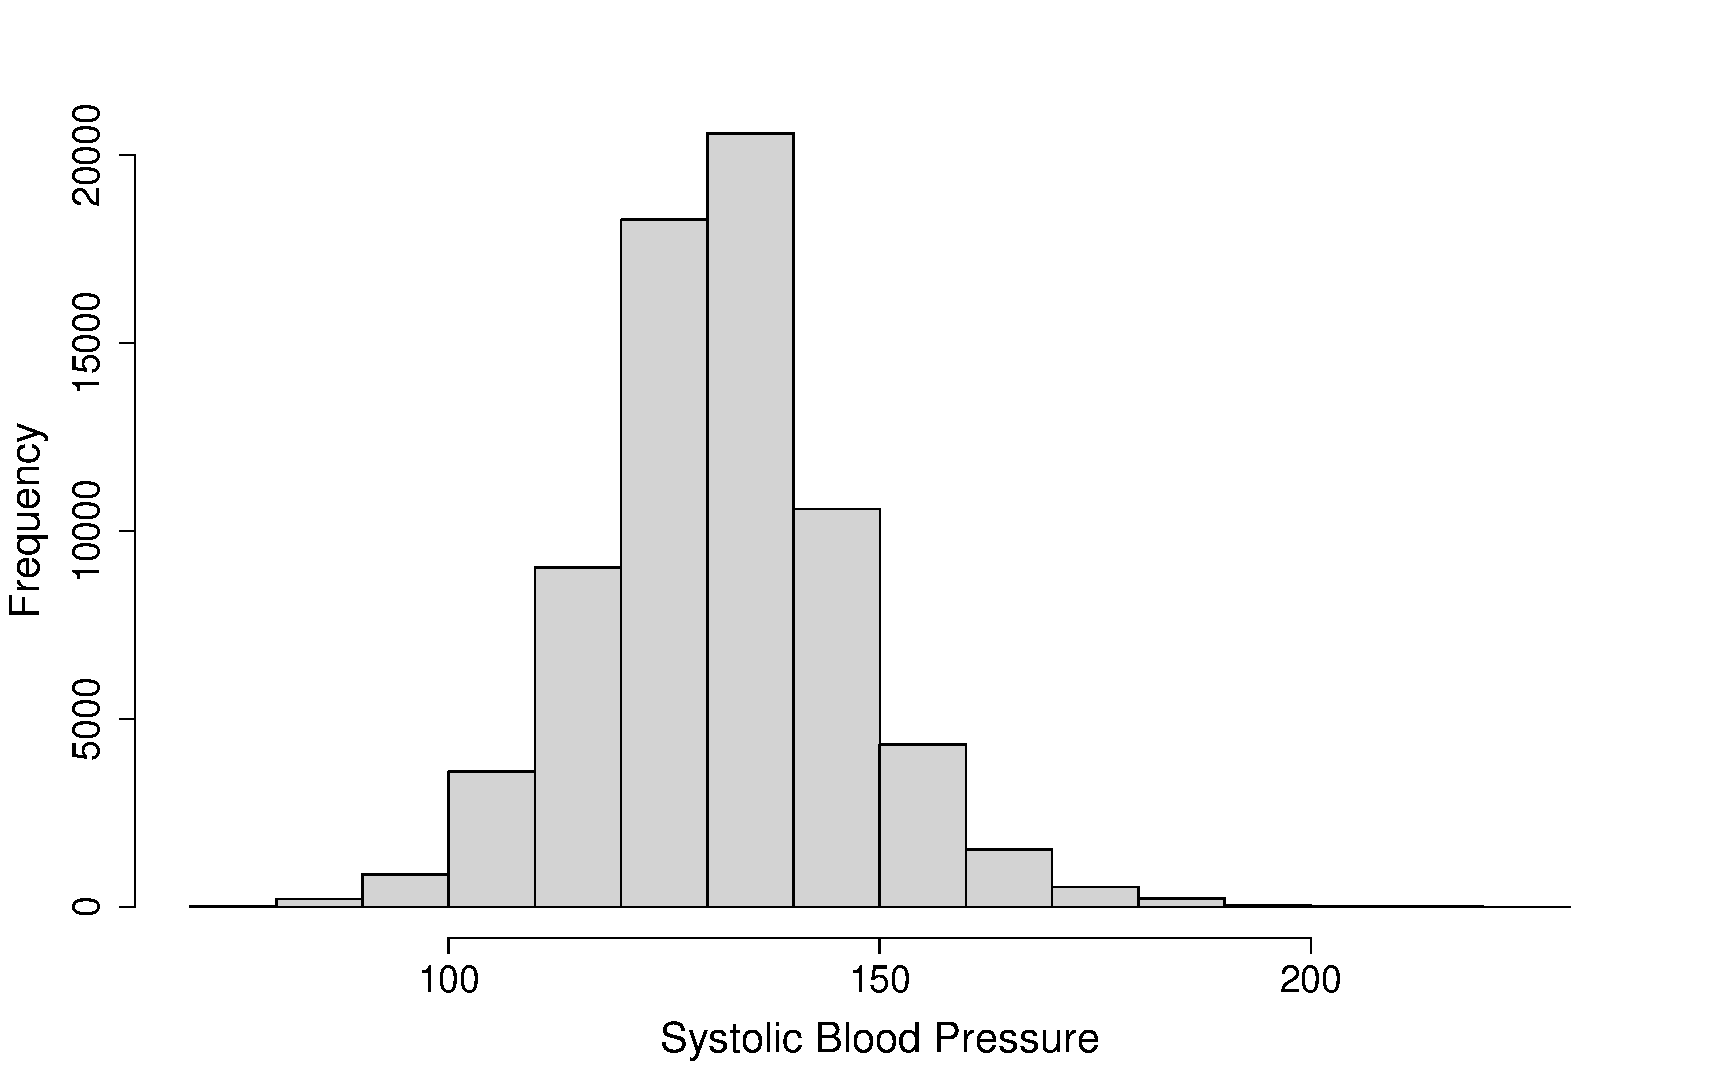
\includegraphics[width=\linewidth]{Images/hist_sys.pdf}
        \caption{Distribution of Systolic blood pressure measures.}
        \label{fig:hist_sys}
     \end{subfigure}
     \hfill
     \begin{subfigure}[b]{0.49\linewidth}
        \centering
        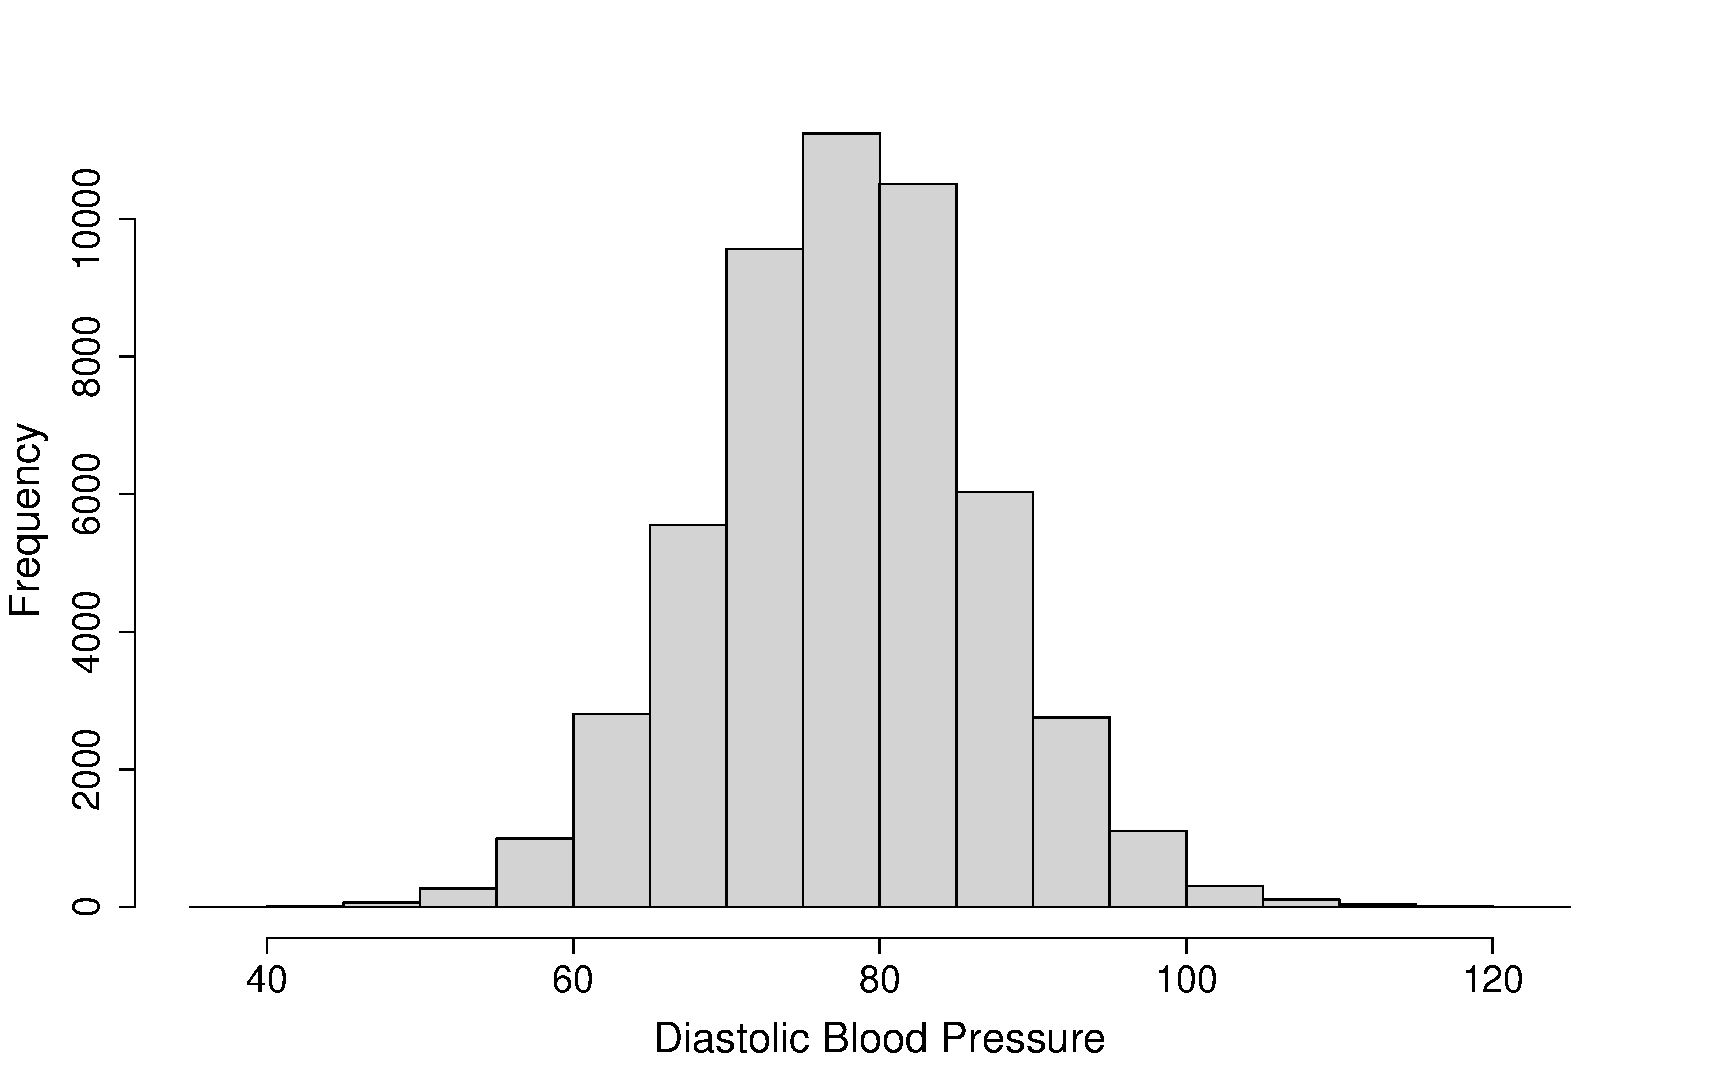
\includegraphics[width=\linewidth]{Images/hist_dia.pdf}
        \caption{Distribution of Diastolic blood pressure measures.}
        \label{fig:hist_dia}
     \end{subfigure}
     \caption{Blood pressure distributions.}
     \label{fig:hist_long}
\end{figure}

\end{frame}

\begin{frame}{Including tables}
You can add tables to the document the same as you do in any latex document.  

\begin{table}[H]
    \centering
    \caption{Intercept and Slope estimates from the linear regression model.}
    \begin{tabular}{rrrr}
    \hline
     & \textbf{Estimate} & \textbf{p-value} & \textbf{95\% CI} \\
    \hline
    \textbf{Intercept} & -1.237 & 0.324 & [-3.026 ; 0.990]\\
    \textbf{Slope} & -7.032 & 0.015 & [-12.555 ; -1.509] \\
    \hline
    \end{tabular}
    \label{tab:reg_est}
\end{table}

\end{frame}


\begin{frame}{Including equations/mathematics}
Numbered:
\begin{equation}
    \hat{y}_i = \hat{\beta}_0 + \hat{\beta}_1 x_{1i} + \hat{\beta}_{2} x_{2i} +...+ \hat{\beta}_p x_{pi}
\end{equation}
or not numbered:
\begin{equation*}
    \hat{y}_i = \hat{\beta}_0 + \hat{\beta}_1 x_{1i} + \hat{\beta}_{2} x_{2i} +...+ \hat{\beta}_p x_{pi}
\end{equation*}

You can also include maths in-line (for example: $\hat{\beta_1} = 0.53$) using dollar signs.

\end{frame}